\documentclass[10pt,a4paper]{article}
\usepackage[margin=.78in]{geometry}\usepackage[T1]{fontenc}
\usepackage{lmodern,microtype,booktabs,graphicx,xcolor,hyperref,xurl,seqsplit}
\hypersetup{hidelinks}\setlength{\parindent}{0pt}\setlength{\parskip}{6pt}
\title{IDM-Viz: Second-Domain Stream Evaluation on ELEC2}
\author{Ahmed Bilal (23I-2581) \and Umar Behram (23I-2604)}\date{16 November 2026}
\begin{document}\maketitle
\begin{abstract}
We evaluated the frozen IDM-Viz monitor on a second external binary stream, OpenML Electricity (ELEC2), using 45,312 records and a coarse time ordering reconstructed from normalized date and period fields. On the final 27,188 observations, row-weighted accuracy was 0.628 and fixed-model calibrated-accuracy MAE averaged 0.059 across 55 cohorts. Input tests alarmed in 55/55 batches. This is a one-domain extension without known drift onset labels; the alarms cannot be scored as drift recall.
\end{abstract}
\section{Source and protocol}
The source is \href{https://www.openml.org/search?id=151}{OpenML dataset 151, version 1} (45,312 records; public dataset visibility), also wrapped as `Elec2` in the \href{https://github.com/online-ml/river/blob/main/river/datasets/elec2.py}{River stream dataset}. OpenML lists Harries (1999), \emph{SPLICE-2 Comparative Evaluation: Electricity Pricing}, and Gama et al. (2004), \emph{Learning with Drift Detection}, DOI \href{https://doi.org/10.1007/978-3-540-28645-5\_29}{10.1007/978-3-540-28645-5\_29}.

The downloaded ARFF source SHA-256 is \texttt{\seqsplit{2d86fbc74c69a5c04bcde0119bce280dd6d8efa0115987edc75b77ccf024d7f2}}. Its row order is not monotone by its normalized date field. We reconstructed a coarse order by normalized date, source order of `(date, weekday)` groups, then period. Eleven normalized date values have multiple weekday groups, so ordering within those ties is approximate. The six model inputs exclude date (ordering only) and contemporaneous NSW price (target-proximal): day, period, NSW demand, Victoria price, Victoria demand and scheduled transfer.

Rows 1--10,800 train the frozen logistic model and training-only scaler/PCA/clusters; rows 10,801--14,462 fit isotonic correctness calibration; rows 14,463--18,124 form the labelled reference; remaining rows are monitored in batches of 500, with a final batch of 188. The input reference is the last 1,000 rows of the reference partition. Six input KS tests plus three frozen PCA tests use within-batch Holm correction at 0.05. Predictions and scores were persisted before label release. Delays 0, 5 and 20 are replayed over identical caches, with post-stream drain.
\section{Results}
Across monitored rows, accuracy was 0.628, balanced accuracy 0.622, and fixed two-class macro-F1 0.604. Equal-batch calibrated-estimate MAE was 0.059, with signed bias -0.011. Row-weighted correctness Brier score was 0.216; equal-batch 10-bin ECE was 0.080. The plug-in interval covered 23/55 realized cohort accuracies. All 55 batches produced an input alarm. This counts observed feature distribution differences, not detections of known concept drift.

At the input end, delay 0 had 55/55 batches verifiable, delay 5 had 50/55, and delay 20 had 35/55; all 55 cohorts release after the respective drain. The final partial batch is retained. Online output contains no current labels, accuracy or correctness.
\begin{figure}[ht]\centering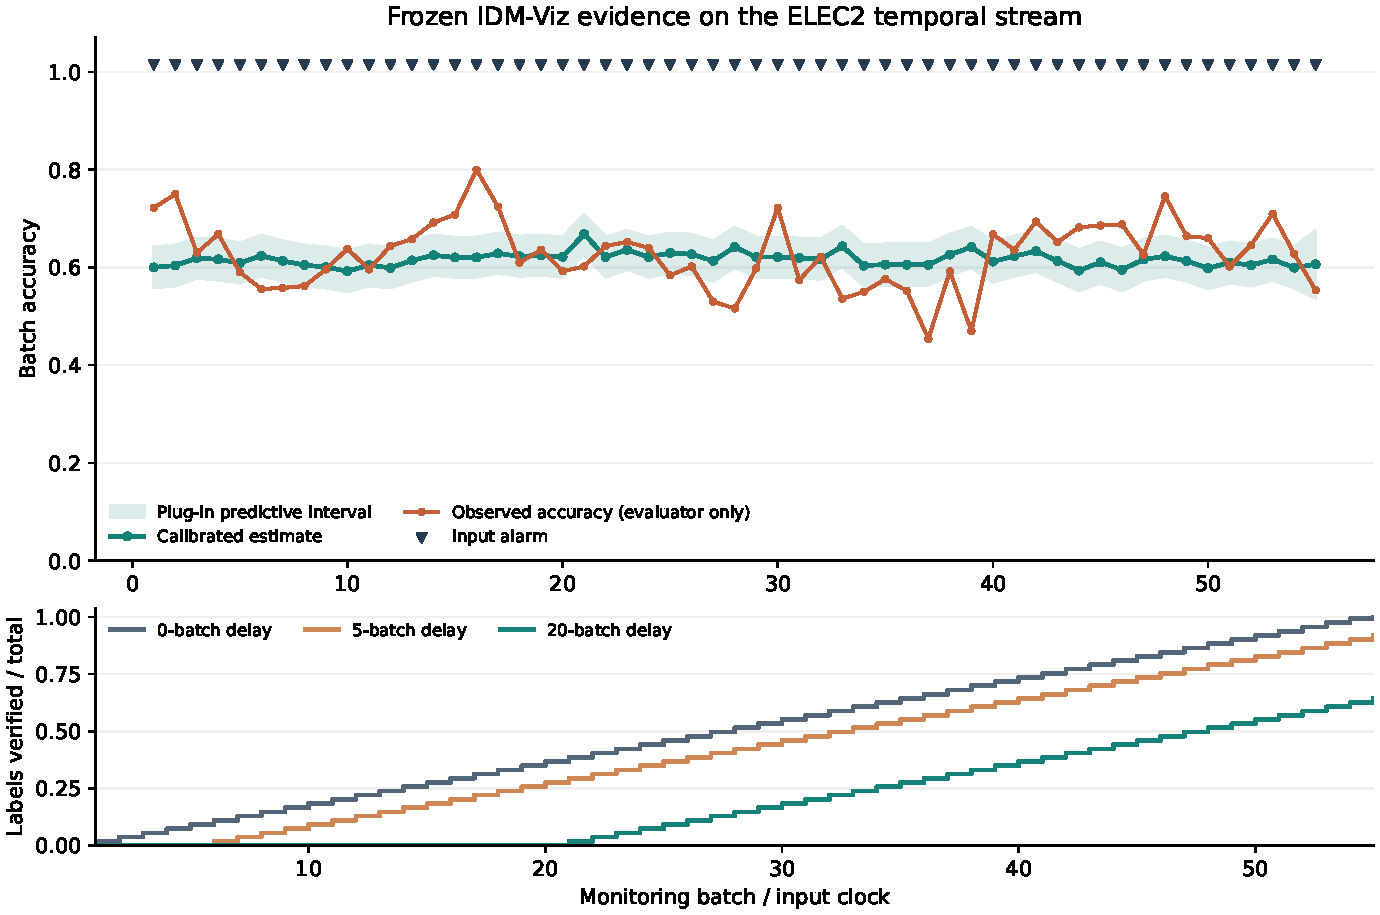
\includegraphics[width=.96\linewidth]{elec2_timeline.pdf}
\caption{Fixed-model estimates, retrospectively observed accuracy, plug-in intervals, input alarms and delayed-label availability in coarse stream order. The lower panel shows the fraction of monitoring labels verified by each input clock.}
\end{figure}
\section{Interpretation and limits}
This second domain adds evidence that the integrated feature/estimate/release pipeline runs beyond the Gas Sensor dataset. It does not establish general transfer: there is one additional domain and one fixed chronological split. The 55/55 input alarms may reflect sustained temporal feature change, but no labeled onset or stationary control exists. The reconstructed normalized-time order has tied groups. Accuracy and calibration outcomes are retrospective evaluation only. The Poisson-binomial interval assumes independent correctness indicators and known calibrated probabilities; batch dependence and calibration/reference uncertainty are omitted. No causal explanation, future-risk forecast or analyst benefit is established.
\section{Reproduction}
\begin{verbatim}
python scripts/run_elec2_temporal_validation.py --out results/phase3/elec2_NEW
python scripts/evaluate_elec2_temporal_validation.py --run results/phase3/elec2_NEW
python scripts/report_elec2_temporal_validation.py
\end{verbatim}
The Phase 2 DOCX and prior result versions remain unchanged.\end{document}
